\section{Results}
\label{sec:result}
\subsection{Multi-wavelength light curves}
\label{sec:multi-lc}%,fig:x-ray-uv-lc-rp-secondaxis,fig:radio-lc
Multi-wavelength light curves of Mrk~1018 are presented in \autoref{fig:multi-lc-secondaxis}. Between 2005 and 2010, when Mrk~1018 stayed in the bright type 1 phase, the X-ray flux was roughly unchanged. The optical/UV flux showed a slight decline by a factor $\sim 1.4 $ during 2005--2007. 

Between 2010 and 2015, both the optical/UV and the X-ray flux showed rapid decay \citep[see also ][]{2016A&A...593L...8M,2016A&A...593L...9H}, and Mrk~1018 changed from type 1 into type 1.9. The optical/UV and X-ray flux declined by a factor of $\sim 17$ and $\sim 7.5$, respectively. 

We find a re-flare (around 2013-2014) during the decay phase, while the amplitude of X-ray variation is higher than those in optical/UV bands (see \autoref{fig:multi-lc-secondaxis}, the X-ray flux increase by a factor $\sim 3$ within $\sim$ 100 days then decrease by a factor of $\sim 4.2$. The optical/UV flux increase by a factor of $\sim 1.5$ within $\sim$ 100 days then decrease by a factor of $\sim 3.8$.). After 2015, the source went into the faint type 1.9 phase. The X-ray showed stronger variability ($\sim $ 14 \%) than optical/UV bands ($\sim $ 6 \%) during the type 1.9 phase in 2018.  

The 5 GHz radio flux did not decline during the decay of X-ray and optical/UV emission between 2010 and 2015 and, however, it decreased by $\sim 20$ \% in the type 1.9 phase during 2016--2017 (see \autoref{fig:multi-lc-secondaxis}).



\begin{figure*}
\centering
	% To include a figure from a file named example.*
	% Allowable file formats are eps or ps if compiling using latex
	% or pdf, png, jpg if compiling using pdflatex
	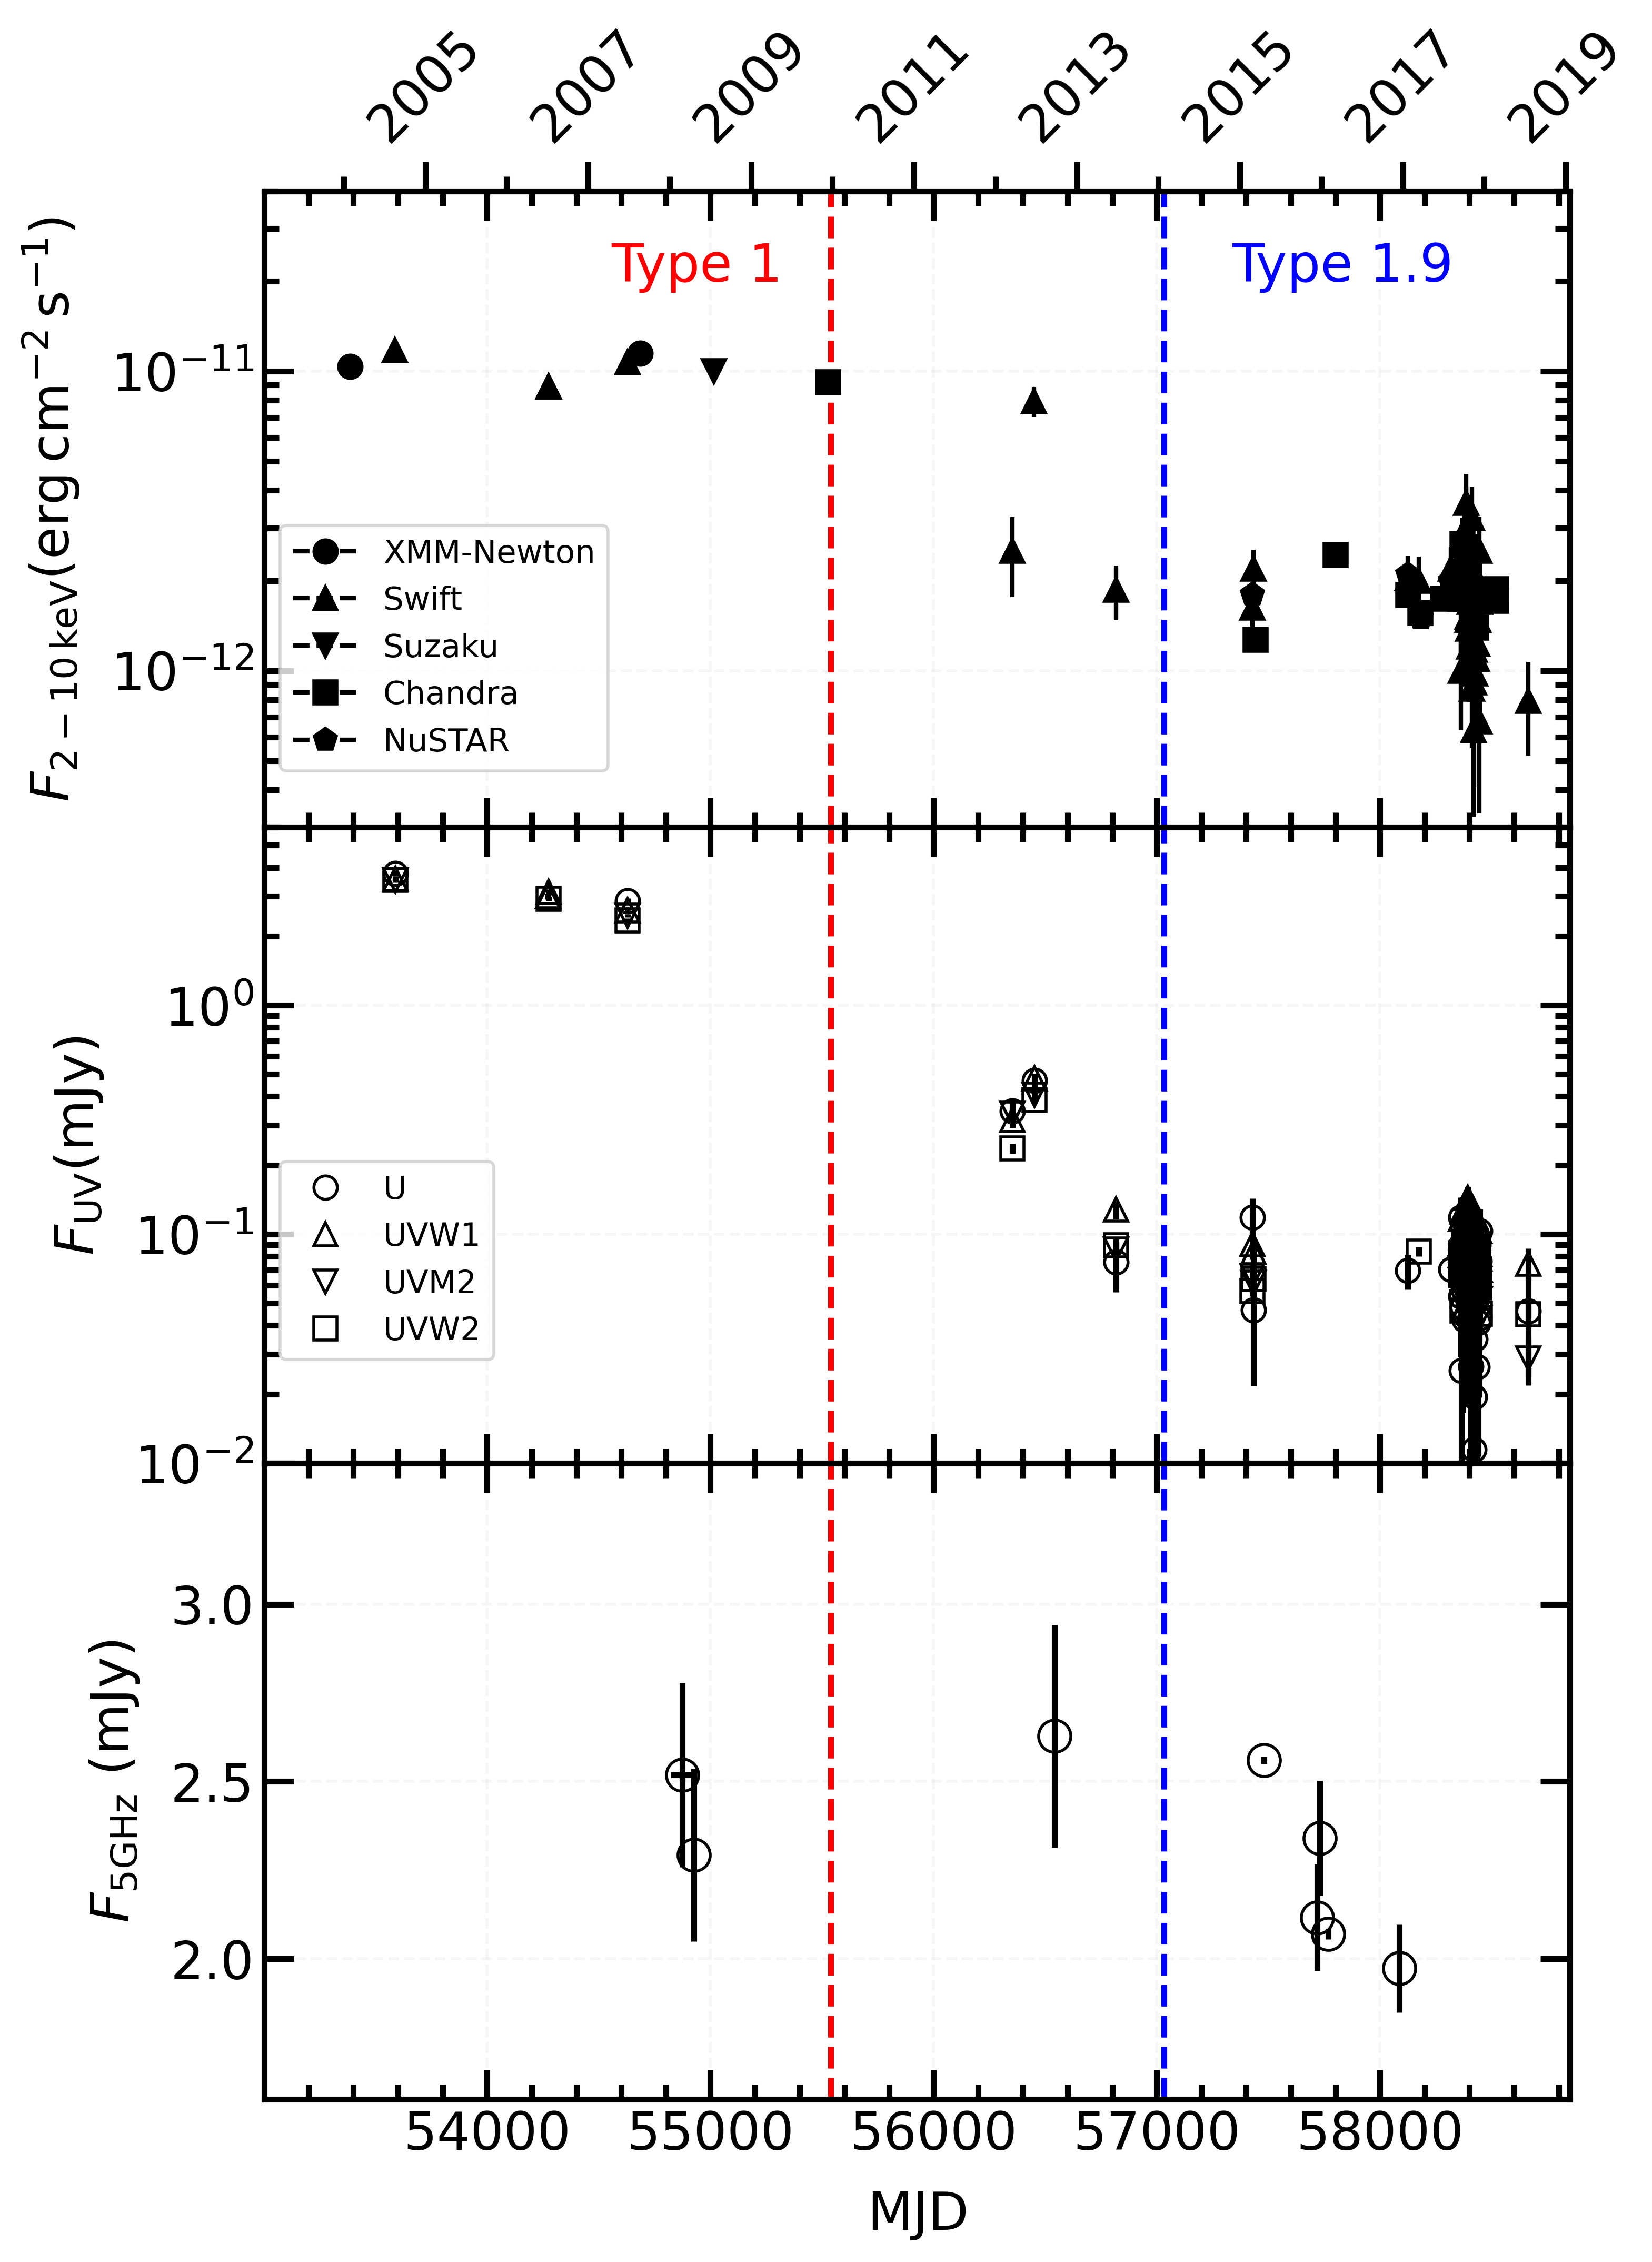
\includegraphics[width=0.9\textwidth]{./pic/subplots-xrt_uvot-radio-second.png}
    \caption{Multi-wavelength light curves of Mrk~1018 between 2005 and 2019. Red and blue vertical dashed lines represent the timeline of optical spectroscopic confirmation at type 1 and type 1.9, respectively. A re-flare during the changing-look phase is found in both the X-ray and the optical/UV bands.}
    \label{fig:multi-lc-secondaxis}
\end{figure*}

\subsection{Time lag between X-ray and UV variations}
Between 2018 August and 2018 November, \swift\, executed a rich monitoring campaign on Mrk~1018 (48 visits within 84 days). In order to examine the correlation between X-ray and UV flux variations during this period, we use the interpolation cross correlation function \citep[ICCF;][]{1998PASP..110..660P} with a time lag ($\tau$) range of 0--40 days (around half the overlap). The interpolation time step of 1 day are both applied to X-ray and UV light curves. The flux randomization and random subset selection methods are employed with 10000 realizations in the Monte Carlo simulation to estimate the centroid time lag and the error \footnote{The code \texttt{pyCCF} is available in \url{http://ascl.net/code/v/1868}}. We find a candidate time lag between X-ray and UVW1 band at $\tau \sim 18.1 ^{+6.5}_{-10.1} $ days (X-ray lead UV) with a correlation coefficient of 0.46 and a $p$-value of 1.3$\times10^{-3}$.

We use the \texttt{JAVELIN} algorithm \citep[][]{2011ApJ...735...80Z,2013ApJ...765..106Z} to further examine the time lag that we estimate through the ICCF method. The \texttt{JAVELIN} approach fits the light curves using a damped random walk (DRW) model, convolves them with a top-hat transfer function (TF), and aligns them to recover the time lag and other parameters (such as the amplitude and timescale of the DRW process, the height and width ($w$) of the top-hat transfer function) with the Monte Carlo method. We first restrict the range of time lag $\tau$ and the $w$ to be 0--40 days. We find a time lag between X-ray and UVW1 band at $\tau \sim 21.4^{+2.2}_{-2.8}$, which is consistent with the results through ICCF method. We find two peaks of the posterior likelihood distribution of $\tau$ ($\sim$ 20 and 32 days) between X-ray and UVM2 band, while the peak at $\sim$ 32 days is higher than that in $\sim$ 20 days. This result does not agree with the ICCF method. So we perform an additional simulation and restrict the range $w$ to be 15--40 days. We find only one peak of the posterior likelihood distribution of $\tau$ at $\sim$ 23 days. 

We estimate the time lag on a magnitude of $\sim $ 20 days between X-ray and UV bands at the 5\% significance level. We cannot distinguish the inter-band time lags in UV bands within errors. We list the detailed time lag analysis results in \autoref{tab:tablelag}.
%\begin{table}
\renewcommand{\arraystretch}{1.5}
\centering
\caption{{\bf Detected time lag $\tau$ of the UV variations behind the X-ray.} The X-ray band is taken as the reference. Errors refer to $1\sigma$ uncertainties.}
\label{tab:tablelag}
\begin{tabular}{lcccccr}
\hline
\hline
 band & method & $\tau$ & correlation coefficient & $p$-value   \\ 
      &        &  [day] &                         &             \\ \hline
U     & ICCF &  $13.4 ^{+17}_{-6} $ & 0.40 & 3.8e-3  \\
UVW1  & ICCF &  $18.1 ^{+6.5}_{-10.1} $ & 0.46 & 1.3e-3 \\
UVM2  & ICCF &  $21.0 ^{+8}_{-5.1} $ & 0.50 & 1.4e-3 \\
UVW2  & ICCF &  $21.0 ^{+6.5}_{-14} $ & 0.37 & 1.7e-2 \\
\hline \hline
band & method & $\tau$ & $w$ range &  $w$  \\ 
     &        &  [day] & [day]  &    [day]  \\ \hline 
U     & \texttt{JAVELIN} &  $ 14.7^{+10.4}_{-8.6} $ & 0--40 & $16.5 ^{+13.4}_{-10.6} $ \\
UVW1  & \texttt{JAVELIN} &  $ 21.4 ^{+2.2}_{-2.8} $  & 0--40 & $9.3 ^{+8.2}_{-5.7} $  \\
UVM2  & \texttt{JAVELIN} &  $ 23.4^{+7.3}_{-9.6} $  & 15--40 &  $ 25.1^{+8.7}_{-7.2} $  \\
UVW2  & \texttt{JAVELIN} &  $ 20.9 ^{+11.4}_{-13.2} $  & 0--40&  $ 12.7 ^{+16.9}_{-10.4} $ \\
\hline \hline
\end{tabular}   
\end{table}


\begin{table}
\renewcommand{\arraystretch}{1.5}
\centering
\caption{{\bf Detected time lag $\tau$ of the UV variations behind the X-ray.} The X-ray band is taken as the reference. Errors refer to $1\sigma$ uncertainties.}
\label{tab:tablelag}
\begin{tabular}{lcccccr}
\hline
\hline
 band & method & $\tau$ & correlation coefficient & $p$-value   \\ 
      &        &  [day] &                         &             \\ \hline
U     & ICCF &  $13.4 ^{+17}_{-6} $ & 0.40 & 3.8e-3  \\
UVW1  & ICCF &  $18.1 ^{+6.5}_{-10.1} $ & 0.46 & 1.3e-3 \\
UVM2  & ICCF &  $21.0 ^{+8}_{-5.1} $ & 0.50 & 1.4e-3 \\
UVW2  & ICCF &  $21.0 ^{+6.5}_{-14} $ & 0.37 & 1.7e-2 \\
\hline \hline
band & method & $\tau$ & $w$ range &  $w$  \\ 
     &        &  [day] & [day]  &    [day]  \\ \hline 
U     & \texttt{JAVELIN} &  $ 14.7^{+10.4}_{-8.6} $ & 0--40 & $16.5 ^{+13.4}_{-10.6} $ \\
UVW1  & \texttt{JAVELIN} &  $ 21.4 ^{+2.2}_{-2.8} $  & 0--40 & $9.3 ^{+8.2}_{-5.7} $  \\
UVM2  & \texttt{JAVELIN} &  $ 23.4^{+7.3}_{-9.6} $  & 15--40 &  $ 25.1^{+8.7}_{-7.2} $  \\
UVW2  & \texttt{JAVELIN} &  $ 20.9 ^{+11.4}_{-13.2} $  & 0--40&  $ 12.7 ^{+16.9}_{-10.4} $ \\
\hline \hline
\end{tabular}   
\end{table}




%\Cref{}
%Radio


\subsection{$\Gamma$-$L_\mathrm{X}/L_\mathrm{Edd}$ and \alphaox- $L_\mathrm{X}/L_\mathrm{Edd}$ correlation}\label{subsec:xray-uv}
We present the $\Gamma$-$\log{L_\mathrm{X}/L_\mathrm{Edd}}$ correlation of Mrk~1018 in \autoref{fig:xrayappendgood-Lrateandg-tmap}, where only the data of \xrt\, are adopted to avoid the discrepancies of different instruments. We find an evident negative correlation between the photon index and the Eddington-scaled X-ray luminosity in the type 1.9 phase, where the Spearman correlation coefficient is $-0.63$ ($p=5.1\times10^{-7}$). The data in the type 1 phase and the re-flare apparently deviate from the negative correlation (see \autoref{fig:xrayappendgood-Lrateandg-tmap}). 

The correlation of $\alpha_{\rm ox}-\log{L_\mathrm{X}/L_\mathrm{Edd}}$ is also explored in \autoref{fig:alpha_ox_lx}. We calculate the $\alpha_{\rm ox}$ according to the \autoref{definition_alpha_ox}. The $L_\mathrm{UVW1}$ is derived from UVW1 filter of the \uvot\ with central wavelength {2600{$\angstrom$}} and full-width at half max of $\sim 683\angstrom$ \citep{2008MNRAS.383..627P}. The $L_\mathrm{2~ keV}$ is calculated according to \autoref{definition_f2eV}, where the $L_\mathrm{2-10~ keV}$ and photon index $\Gamma$ are derived from X-ray spectra fitting. 
%\begin{equation}
%\alpha_{OX}  = - \frac{\log(\lambda F_{2500 \angstrom}/\nu F_{2keV})}{\log(\nu_{ 2500 \angstrom }/\nu_{2keV})}+1
%\end{equation}
\begin{equation}
\alpha_\mathrm{ox} = \frac{\log (L_\mathrm{UVW1} / L_\mathrm{2keV} )} {\log (\nu_\mathrm{2keV} /  \nu_\mathrm{UVW1} )}=0.384\times {\log (L_\mathrm{UVW1} / L_\mathrm{2keV} )}
\label{definition_alpha_ox}
\end{equation}
%and the $L_\mathrm{2keV}$ is estimated from
\begin{eqnarray}
\large{
L_\mathrm{2~keV}= 
\begin{cases}\displaystyle\frac{L_\mathrm{2-10~ keV} (2-\Gamma)}{\nu_\mathrm{2~keV} \times (5^{2-\Gamma}-1)} \quad &, 
\Gamma \neq 2 \\ 
\displaystyle\frac{L_\mathrm{2-10~ keV}}{\nu_\mathrm{2~keV} \times \mathrm{ln} 5}\quad  &, \Gamma = 2
\end{cases} }
\label{definition_f2eV}
\end{eqnarray} 
The \alphaox\, and $\log{L_\mathrm{X}/L_\mathrm{Edd}}$ also follow a negative correlation in the type 1.9 phase, where the Spearman correlation coefficient is $-0.67$ ($p=1.7\times10^{-7}$). The data in type 1 phase and the re-flare also apparently deviate from the negative correlation (\autoref{fig:alpha_ox_lx}).
 
\begin{figure}
\centering
	% To include a figure from a file named example.*
	% Allowable file formats are eps or ps if compiling using latex
	% or pdf, png, jpg if compiling using pdflatex
	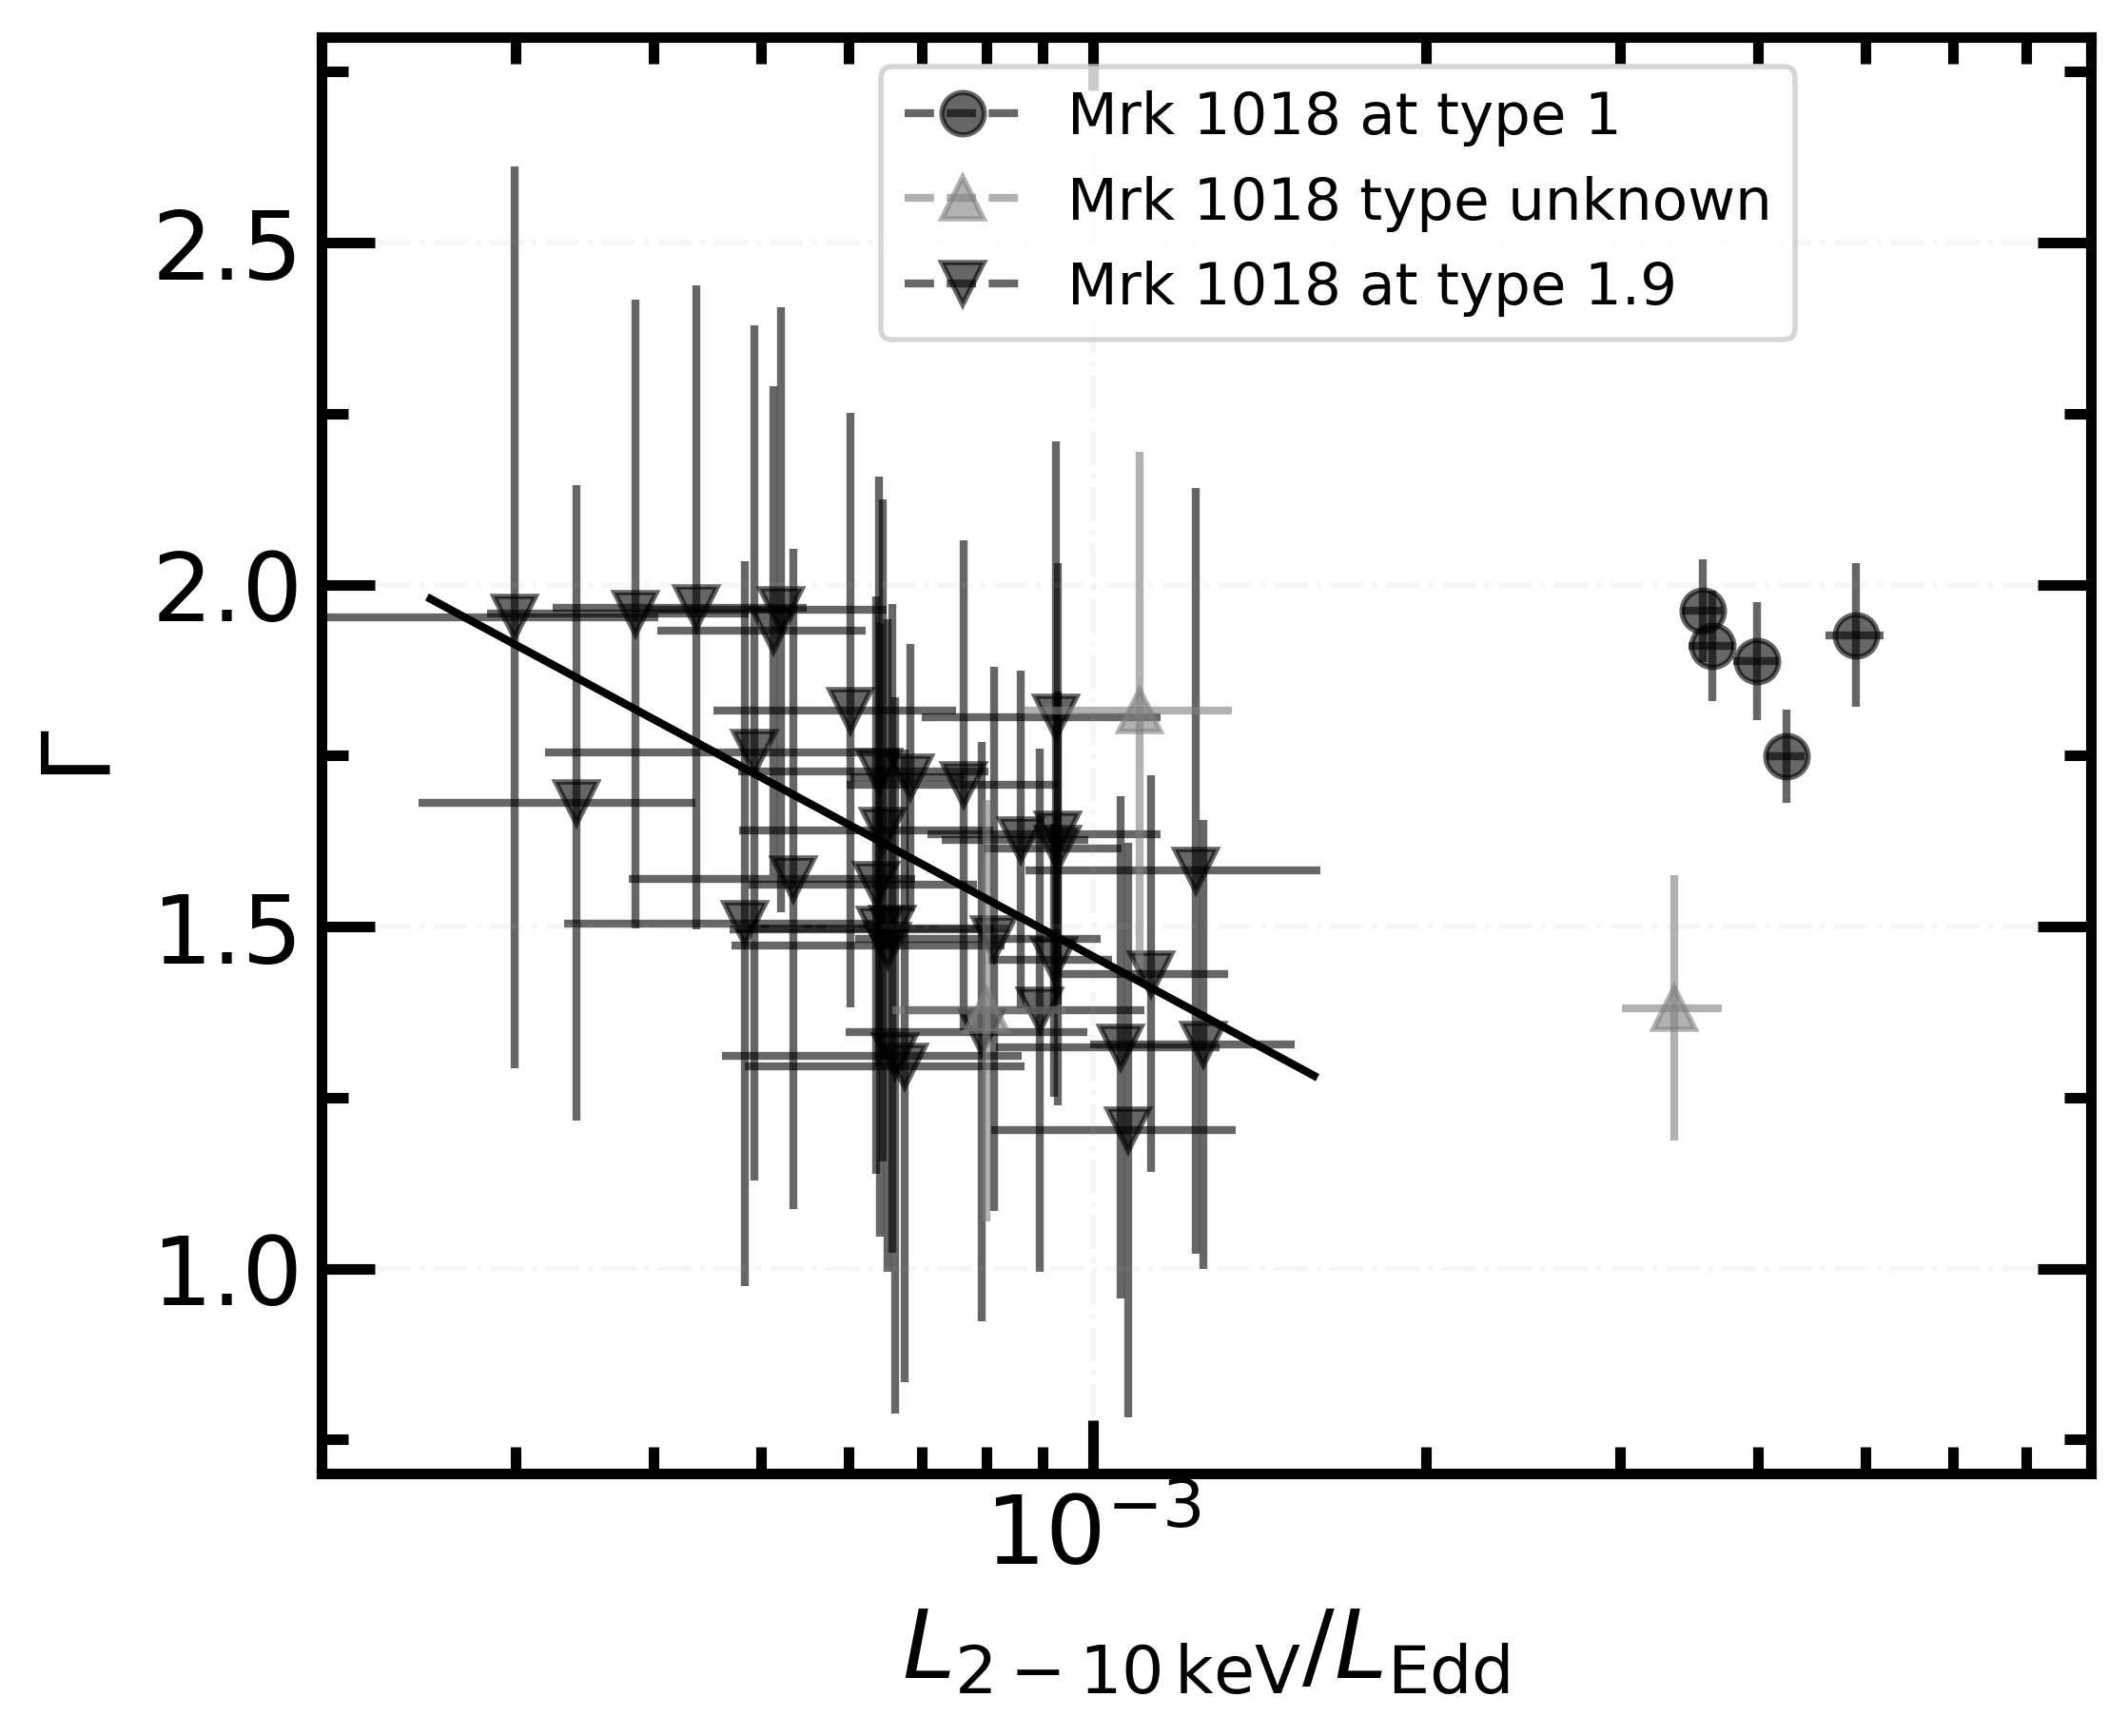
\includegraphics[width=\linewidth]{./pic/xrt_only-errorbar-Lrate-g-tmap_brokenlinear_dot.png}
    \caption{The $\Gamma$ - $L_\mathrm{X}/L_\mathrm{Edd}$ correlation. Only data of \xrt\, are included here. The dashed line represent the best fitting of the negative correlation in the type 1.9 phase.}
    \label{fig:xrayappendgood-Lrateandg-tmap}
\end{figure}
\begin{figure}
\centering
	% To include a figure from a file named example.*
	% Allowable file formats are eps or ps if compiling using latex
	% or pdf, png, jpg if compiling using pdflatex
	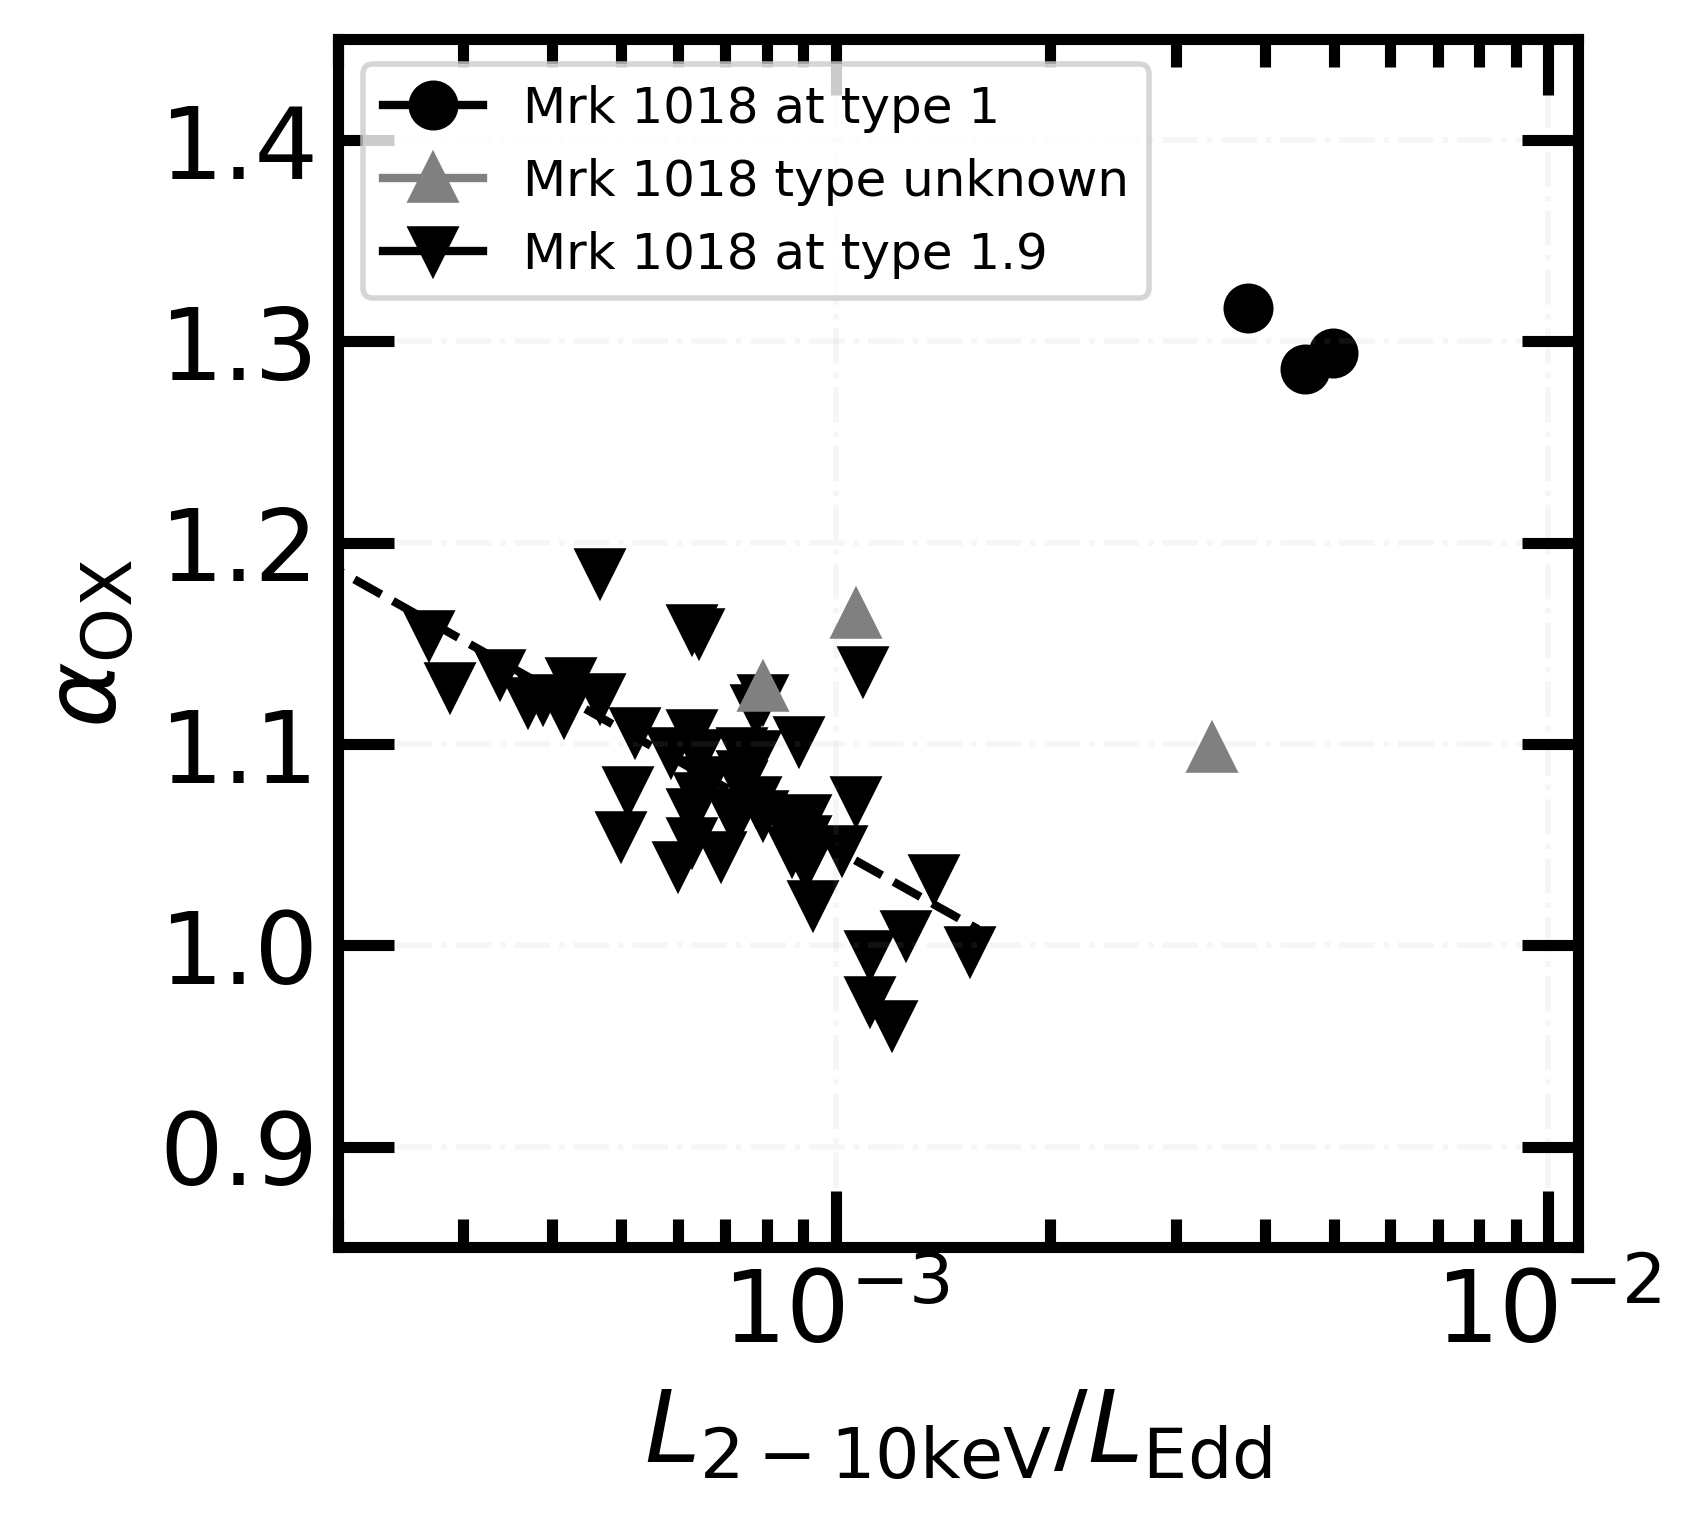
\includegraphics[width=\linewidth]{./pic/Mrk1018_2individuals_alpha_ox_L2-10.png}
    \caption{The $\alpha_\mathrm{OX}-L_{\mathrm{X}}/L_\mathrm{Edd}$ correlation. The dashed line represent the best fitting of the negative correlation in the type 1.9 phase.}   
    \label{fig:alpha_ox_lx}
\end{figure}


\subsection{Radio--X-ray luminosity correlation}
The correlation of the 5 GHz radio luminosity ($\log L_\mathrm{R}$) and 2--10~keV X-ray luminosity ($\log L_\mathrm{X}$) is presented in \autoref{fig:radio-xray-mass_relation_Plotkin2012}, where the quasi-simultaneous radio and X-ray observations within 100 days are adopted. The radio and X--ray luminosity follow a quite flat correlation during the luminosity range of $L_\mathrm{X}/L_\mathrm{Edd}$ $\sim$ 5$\times 10^{-4}$-- 4$\times 10^{-3}$, where the Spearman correlation coefficient is $0.2$ ($p=0.75$). Coincidently, the two points in 2017 and average of the $\log L_\mathrm{R}$ and $\log L_\mathrm{X}$ correlation of Mrk 1018 roughly follows the fundamental plane defined by the sample of AGN and XRB \citep[e.g.][]{2012MNRAS.419..267P}. But the points before 2016 deviate the fundamental plane where $L_\mathrm{R}\propto L_\mathrm{X}^{0.6}$.




\begin{figure}
\centering
	% To include a figure from a file named example.*
	% Allowable file formats are eps or ps if compiling using latex
	% or pdf, png, jpg if compiling using pdflatex
	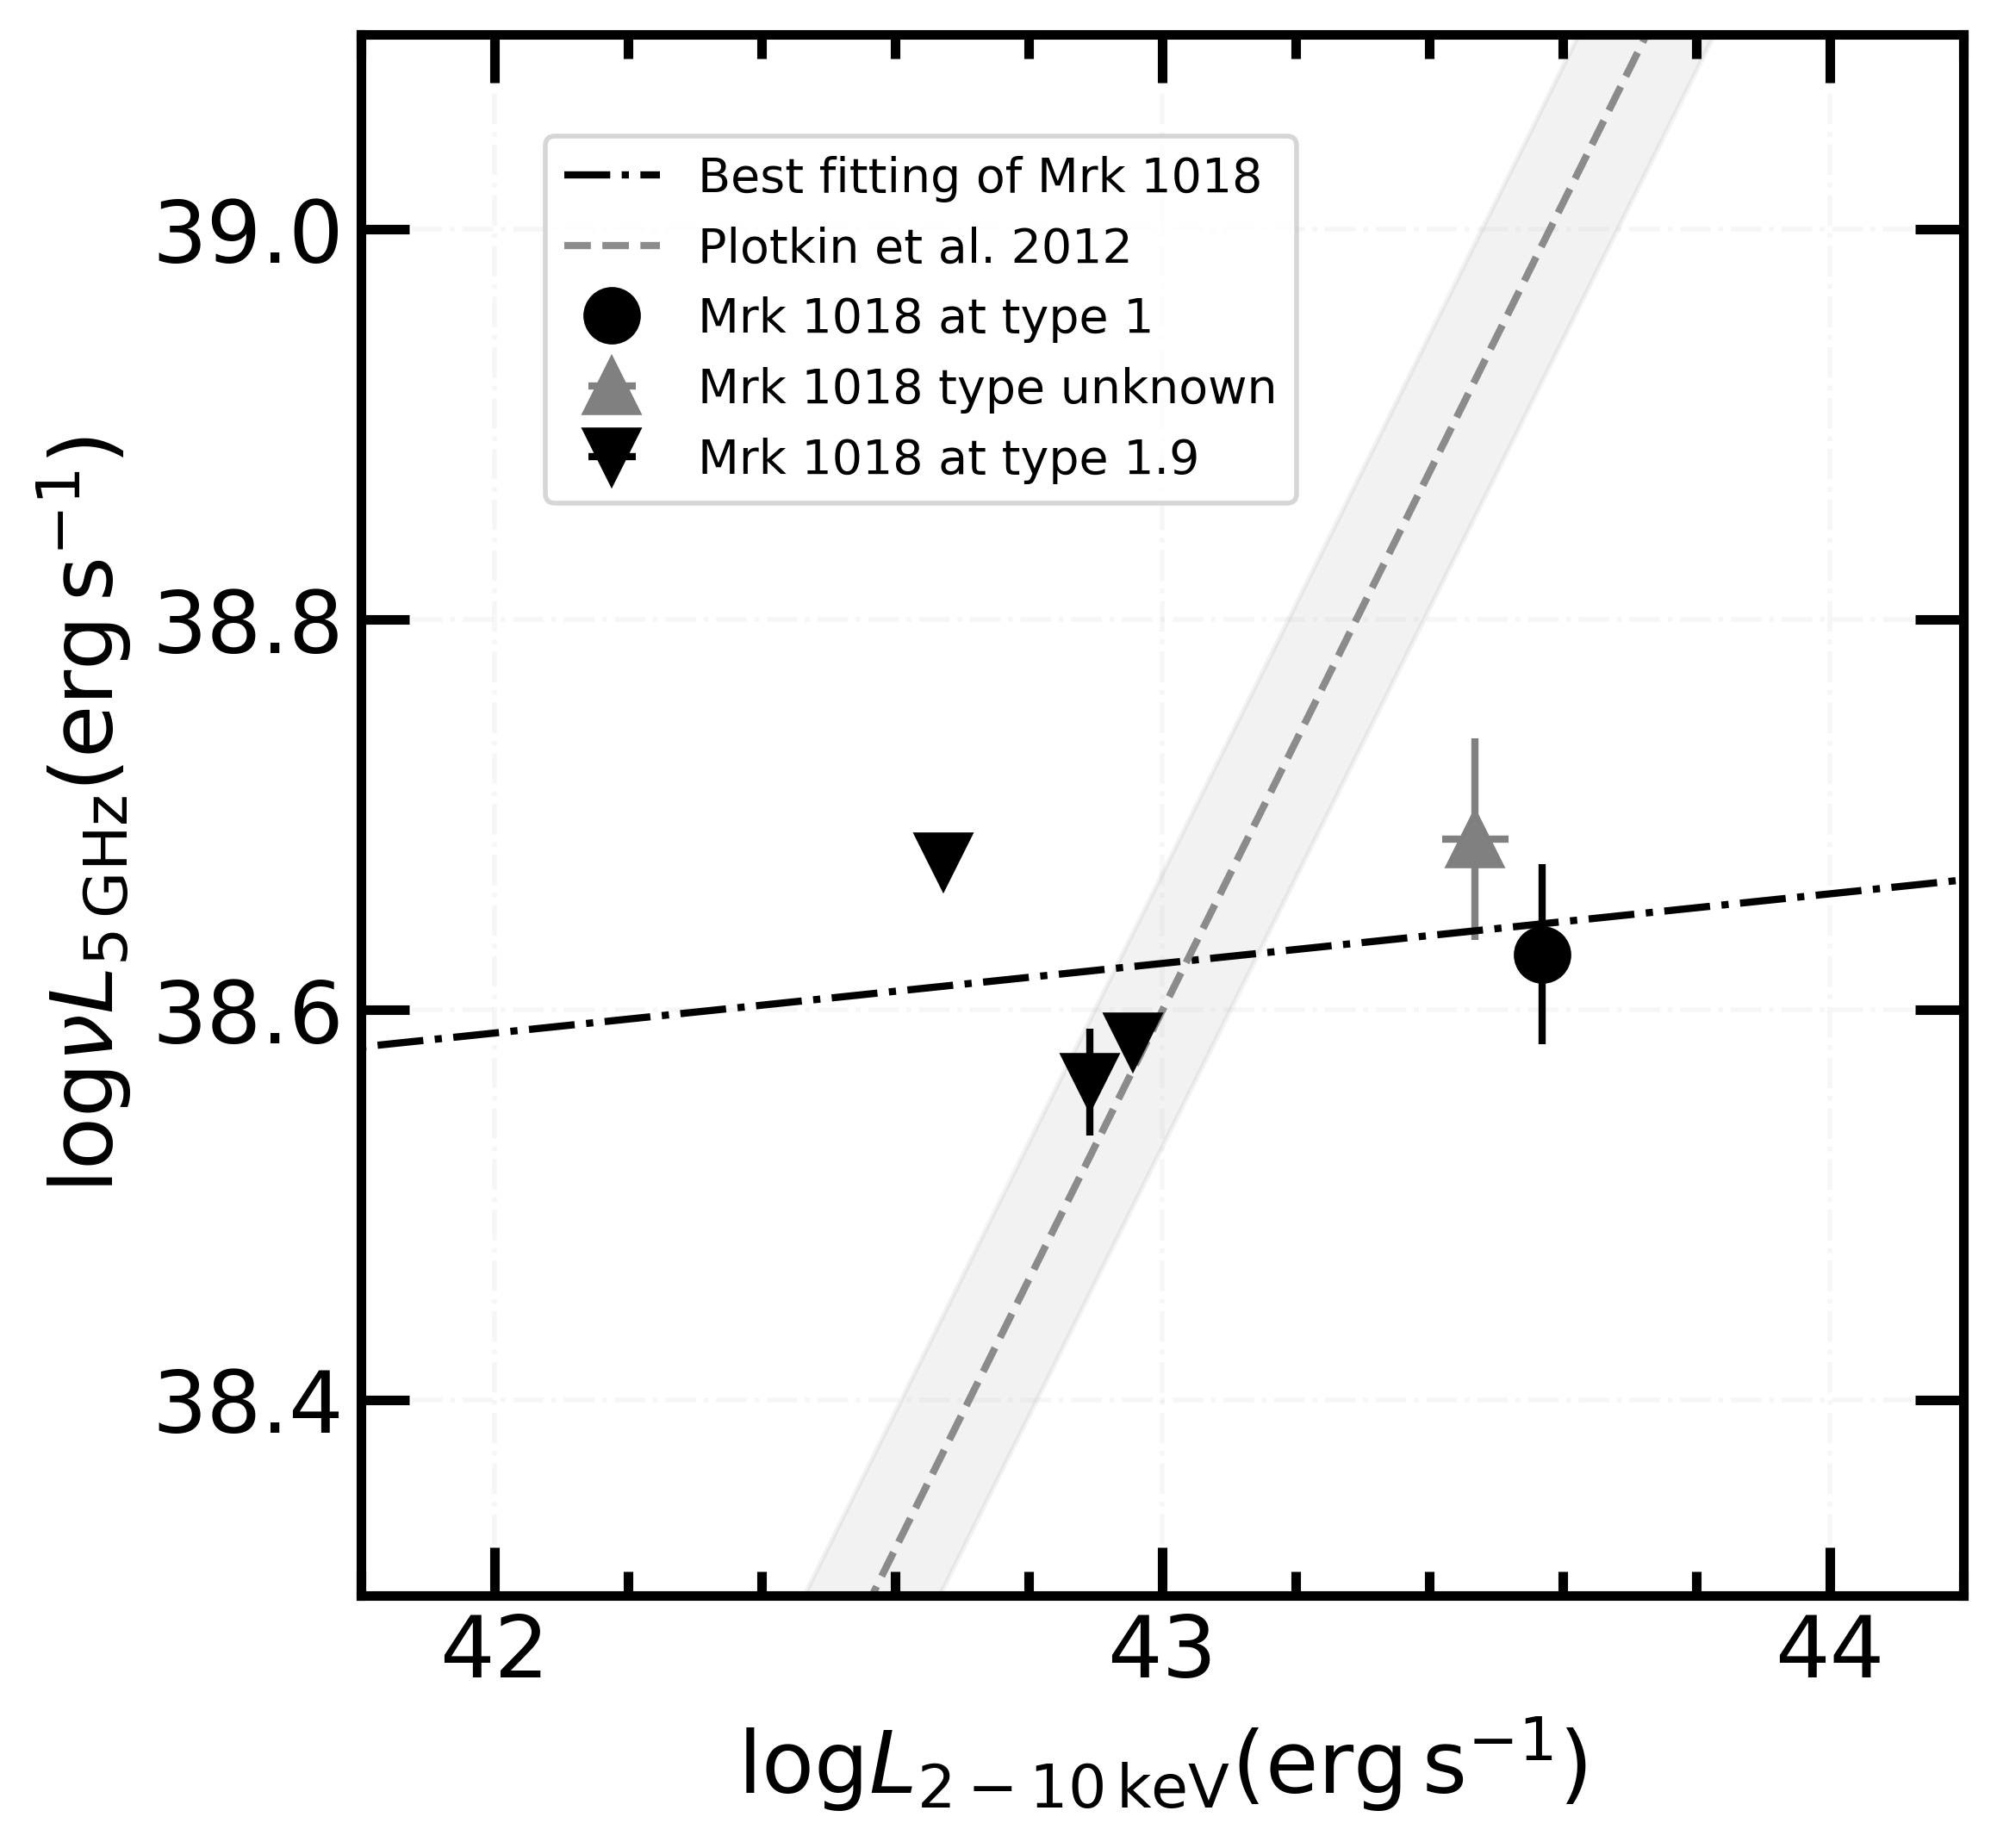
\includegraphics[width=\linewidth]{./pic/Mrk1018_radio_xray_Plotkin2012_Lx_near.png}
    \caption{The $\log L_\mathrm{R}$-$\log L_\mathrm{X}$ correlation. The dash-dot line represents the best-fitting line of Mrk~1018 with a slope of $\sim 0.04$. %The cross point represents the mean value of the radio and X-ray luminosity with the standard deviation as uncertainty. 
    The fundamental plane of a sample of black holes in \citet{2012MNRAS.419..267P} with a slope of $\sim 0.6$ is presented in the grey dashed line with intrinsic $\sigma=0.07$ for comparison.} 
    \label{fig:radio-xray-mass_relation_Plotkin2012}
\end{figure}